\begin{frame}{$\text{LTL}_f\text{/LDL}_f$ Non-Markovian Rewards}
    $\text{LTL}_f\text{/LDL}_f$ non-Markovian rewards + integration
    in our project.
    \begin{figure}
        \centering
        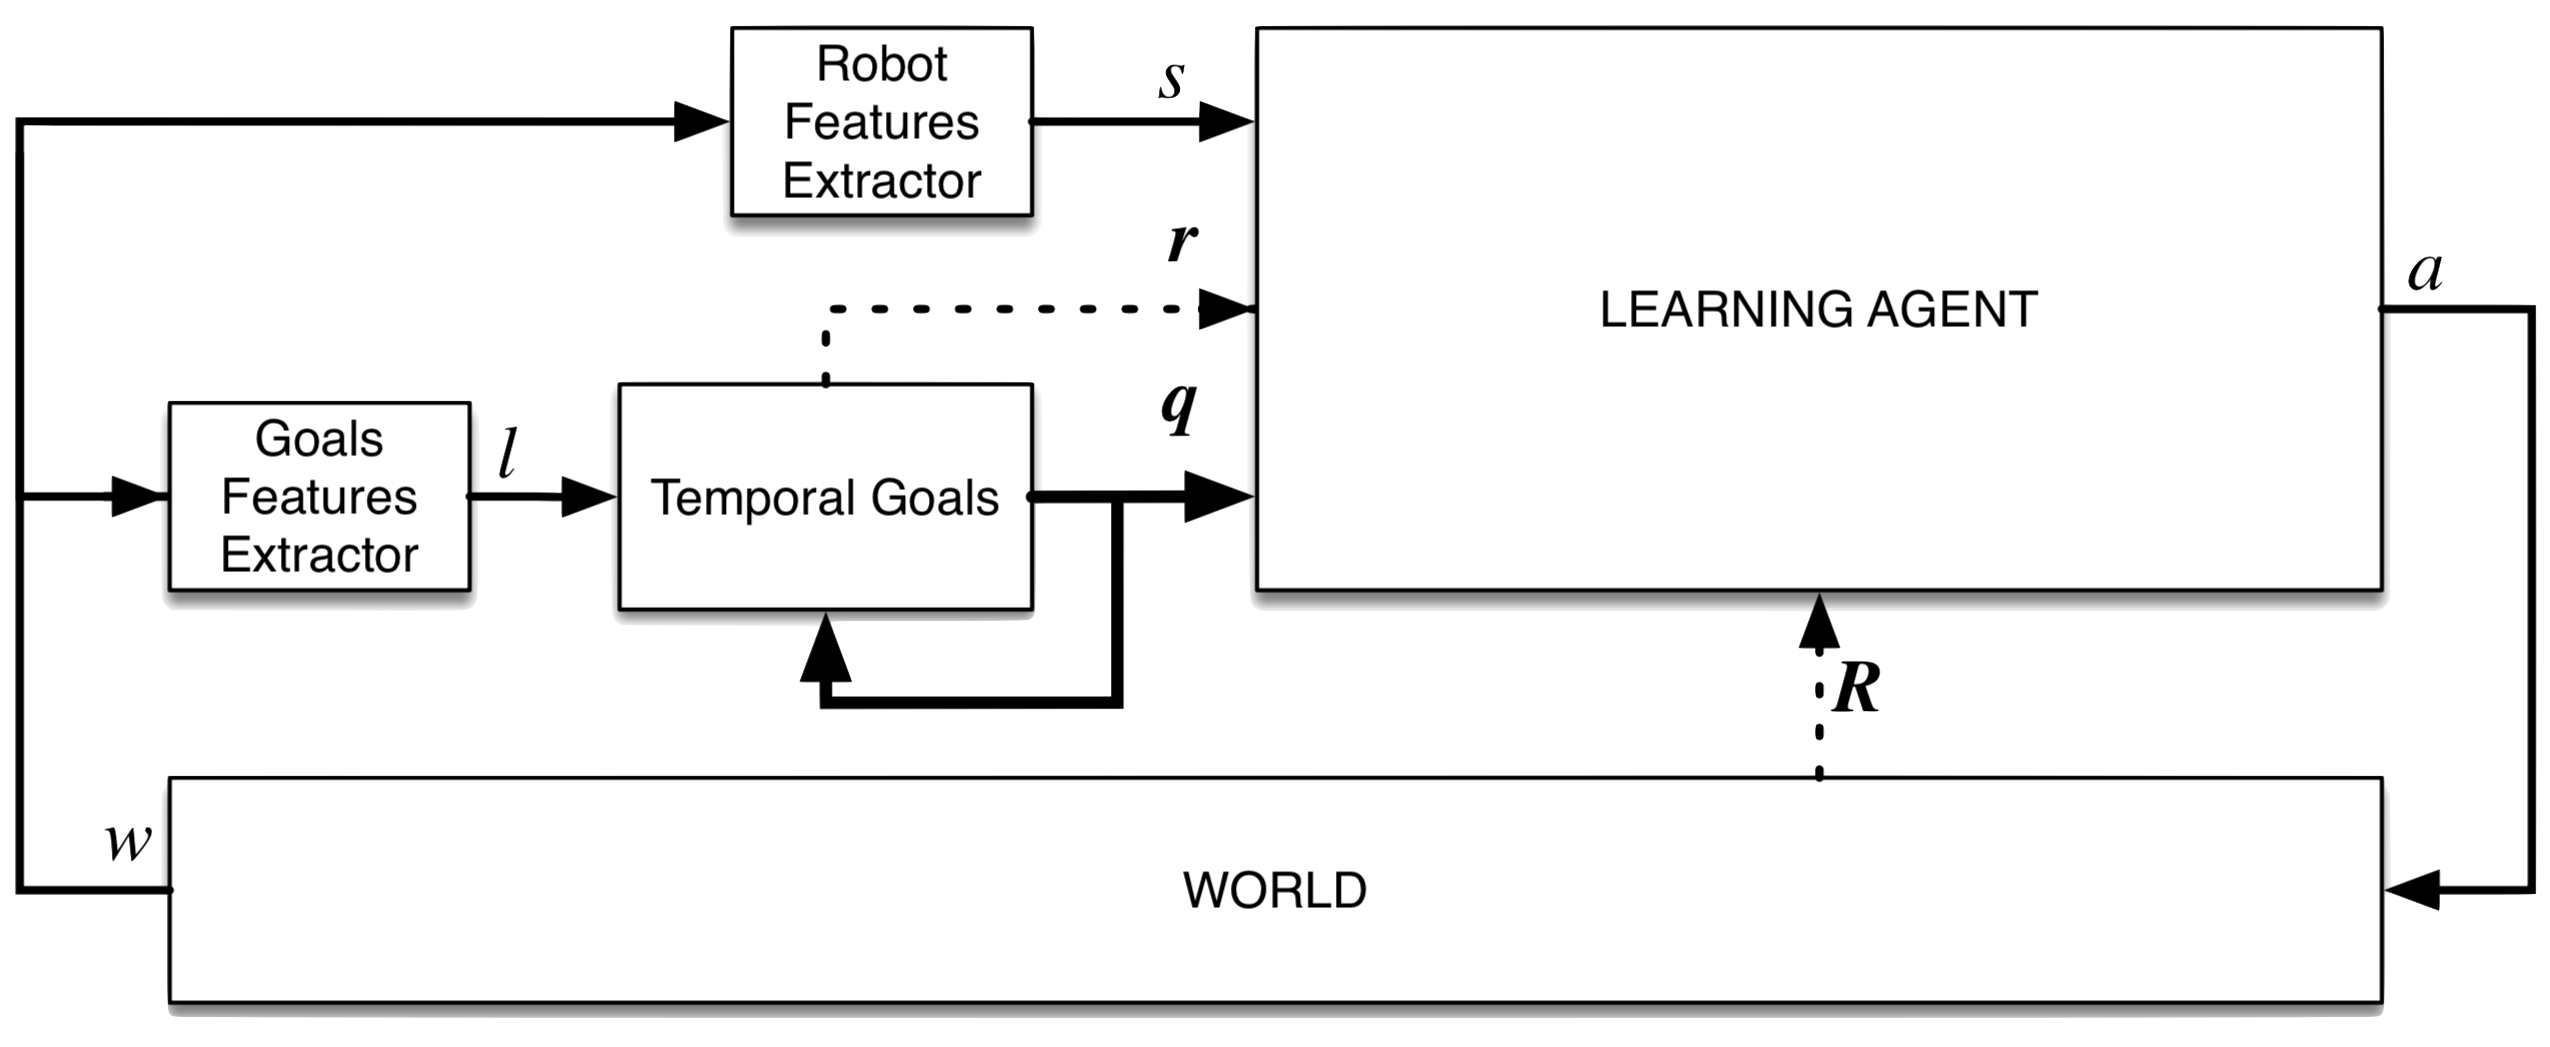
\includegraphics[width=0.95\textwidth]{images/rl-temporalgoals-pipeline.png}
        \caption{Pipeline describing how the agent is interacting with the
            world and how the robot features extractor and the goal features
            extractor are used in order to handle non-Markovian rewards.}
        \label{fig:rl-temporalgoals-pipeline}
    \end{figure}
\end{frame}

\begin{frame}{$\text{LTL}_f\text{/LDL}_f$ Non-Markovian Rewards}
	\begin{block}{}
		Reward for destroying the block rows in order from top to bottom.
		\begin{align*}
		\begin{split}
		\langle&(\neg\varphi_0 \land \neg\varphi_1 \land \neg\varphi_2)^*;
		(\varphi_0 \land \neg\varphi_1 \land \neg\varphi_2);
		(\varphi_0 \land \neg\varphi_1 \land \neg\varphi_2)^*;\\
		&(\varphi_0 \land \varphi_1 \land \neg\varphi_2);
		(\varphi_0 \land \varphi_1 \land \neg\varphi_2)*;
		(\varphi_0 \land \varphi_1 \land \varphi_2)\rangle tt
		\end{split}
		\end{align*}
		where $\varphi_i$ indicates the $i$-th row.
	\end{block}
	
	\begin{block}{}
		\begin{align*}
			(\neg\varphi_0\land \neg\varphi_1\land\neg\varphi_2)&^*
			\text{\quad all rows not destructed for an indefinite amount of time.} \\
			(\varphi_0 \land \neg\varphi_1 \land \neg\varphi_2)&\ 
			\text{\quad first row destructed, other still there.}\\	
		\end{align*}
	\end{block}
\end{frame}


\begin{frame}{$\text{LTL}_f\text{/LDL}_f$ Non-Markovian Rewards}
	\begin{block}{}
		$\text{LTL}_f\text{/LDL}_f$ transformed to an equivalent automaton.
	\end{block}
	\begin{block}{}
		Automaton representation given in input to the learning agent.
	\end{block}
	\begin{block}{}
		Learning agent input:
		$\langle\text{environment state, automaton state}\rangle$
	\end{block}
\end{frame}